\documentclass[11pt,letterpaper]{article}
\usepackage[T1]{fontenc}
\usepackage{lmodern}
\usepackage[margin=1in]{geometry}
\usepackage{amsmath,amssymb,amsthm,mathtools}
\usepackage{enumitem}
\usepackage{microtype}
\usepackage{tikz}
\usepackage[colorlinks=true,linkcolor=blue,citecolor=blue,urlcolor=blue]{hyperref}
\usepackage{bookmark}
\pdftrailerid{}
\pdfsuppressptexinfo=15

\newtheorem{theorem}{Theorem}[section]
\newtheorem{proposition}[theorem]{Proposition}
\newtheorem{lemma}[theorem]{Lemma}
\newtheorem{corollary}[theorem]{Corollary}
\theoremstyle{definition}
\newtheorem{definition}[theorem]{Definition}
\theoremstyle{remark}
\newtheorem{remark}[theorem]{Remark}
\numberwithin{equation}{section}
\setlist{itemsep=3pt,topsep=5pt}
\hypersetup{pdftitle={Talagrand's discrete-convexity conjecture},
  pdfauthor={OpenAI},
  pdfsubject={A positive solution to Talagrand's Research Problem 13.3.2}}

\title{Talagrand's discrete-convexity conjecture}
\author{OpenAI}
\date{September 23, 2026}

\AddToHook{cmd/thebibliography/after}{\addcontentsline{toc}{section}{\refname}}

\begin{document}
\maketitle
\begin{abstract}
We prove Talagrand's discrete-convexity conjecture.
There is a universal integer $k$ such that, whenever an arbitrary family has
Bernoulli product measure at least $1-1/k$, the sets not contained
in a union of $k$ members admit a cover of total cost at most $1/2$
at the same density.
\end{abstract}

\section{Introduction}
\label{sec:introduction}

Let $[N]=\{1,\ldots,N\}$, and let $\mu_p$ be the probability measure
on $2^{[N]}$ under which each coordinate is present independently with
probability $p\in(0,1)$. For a family $\mathcal D\subseteq2^{[N]}$ and
an integer $k\ge1$, define
\begin{equation}
\label{eq:exceptional-definition}
E_k(\mathcal D)
=\bigl\{S\subseteq[N]:
  S\nsubseteq D_1\cup\cdots\cup D_k
  \text{ for all }D_1,\ldots,D_k\in\mathcal D\bigr\}.
\end{equation}
The members in a tuple may repeat and need not be disjoint.

A family $\mathcal G\subseteq2^{[N]}$ \emph{covers} a family
$\mathcal A$ if every $S\in\mathcal A$ contains some $I\in\mathcal G$.
For $\rho\in(0,1)$, write
\[
c_\rho(\mathcal G)=\sum_{I\in\mathcal G}\rho^{|I|}.
\]
We say that $\mathcal A$ is \emph{$p$-small} if it has a cover
$\mathcal G$ with $c_p(\mathcal G)\le1/2$.
Since $\mu_p\{S:I\subseteq S\}=p^{|I|}$, such a cover witnesses
$\mu_p(\mathcal A)\le1/2$ by a union bound.

The name reflects the analogy with Talagrand's Gaussian convexity
question~\cite[Conjecture~2.1]{Talagrand10}: can a bounded number of
sums of a compact balanced set of sufficiently large Gaussian measure
contain a convex set of Gaussian measure at least $1/2$, uniformly in
the dimension? Here balanced means closed under multiplication by
scalars of absolute value at most one. In the discrete problem, unions
replace sums, and containment covers describe the exceptional sets.
Talagrand formulated the discrete-convexity conjecture in
\cite[Conjecture~7.1]{Talagrand10}: a fixed number of members of a
sufficiently likely family should cover every set outside a $p$-small
exceptional family. The same original-density formulation appears as
Research Problem~13.3.2 in~\cite{Talagrand21}, whose
Proposition~13.3.3 explains its connection to positive selector processes.
We prove this conjecture.

\begin{theorem}
\label{thm:main}
Set $k=2^{75}$. For every integer $N\ge1$, every $p\in(0,1)$, and every
family $\mathcal D\subseteq2^{[N]}$,
\[
\mu_p(\mathcal D)\ge1-\frac1k
\quad\Longrightarrow\quad
E_k(\mathcal D)\text{ is }p\text{-small}.
\]
\end{theorem}

The constant is independent of $N$, $p$, and $\mathcal D$.
The family $\mathcal D$ is arbitrary; no monotonicity is assumed.

\paragraph{Positive selectors.}
The connection to positive selector processes
\cite[Section~7]{Talagrand10}
gives a concrete consequence of the theorem, recovering the
positive-selector conclusion proved by Park and Pham
\cite[Theorem~1.2]{ParkPham24}. For a nonempty family
$T\subseteq[0,\infty)^N$, define
\[
\phi(S)=\sup_{t\in T}\sum_{i\in S}t_i,
\qquad M=\mathbb E_{\mu_p}\phi,
\]
and suppose $0<M<\infty$. Then
$\{S:\phi(S)\ge k^2M\}$ is $p$-small for $k=2^{75}$.
Indeed, Markov's inequality gives
$\mu_p\{D:\phi(D)<kM\}\ge1-1/k$.
Nonnegativity of the coordinates makes $\phi$ monotone and subadditive
under unions, so a set with $\phi(S)\ge k^2M$ cannot be contained in
the union of $k$ such $D$'s. Theorem~\ref{thm:main} supplies its cover.
Thus the large-value event has explicit containment witnesses, beyond
the small probability already supplied by Markov's inequality.

\paragraph{Related developments.}
Hua, Song, and Tudose resolve Talagrand's Gaussian convexity problem and
derive a discrete conclusion with three unions and covering density
$p^C$, for a universal constant $C$, when the starting family is
sufficiently likely~\cite[Corollaries~1.3--1.4]{HuaSongTudose26}.
Ascoli, He, Park, and Talagrand give a threshold reformulation of discrete
convexity and prove cases for several graph-containment
properties~\cite[Proposition~1.5 and Theorems~1.10--1.13]{AscoliEtAl26}.

There is also a fractional version of smallness: instead of selecting
generators, one assigns nonnegative coefficients $a_I$ satisfying
\[
\sum_{I\subseteq S}a_I\ge1\quad(S\in\mathcal A),
\qquad
\sum_{I\subseteq[N]}p^{|I|}a_I\le\frac12.
\]
Talagrand introduced this relaxation alongside integral
smallness~\cite[Sections~6 and~7]{Talagrand10}.
Li resolves the fractional discrete-convexity problem through a quantitative
obstruction to probability measures whose containment probabilities
are bounded by $p^{|I|}$~\cite[Theorem~1.9]{Li26}.
Combining fractional information with rounding, Park obtains an integral
cover of $E_2(\mathcal D)$ at density
\[
\frac{p}{C\max\{1,\log\log(1/p)\}}
\]
whenever $\mu_p(\mathcal D)>1/2$, for a universal
$C$~\cite[Corollary~3.5]{Park26}.
Combining Li's result with the companion constant-factor rounding theorem
gives the following two-union tradeoff.

\begin{corollary}[Two unions at constant density loss]
\label{cor:two-union}
There is a universal constant $C\ge1$ such that, for every integer $N\ge1$,
every $p\in(0,1)$, and every family $\mathcal D\subseteq2^{[N]}$,
\[
\mu_p(\mathcal D)>\frac12
\quad\Longrightarrow\quad
E_2(\mathcal D)\text{ is }(p/C)\text{-small}.
\]
\end{corollary}

\begin{proof}
If $E_2(\mathcal D)=\varnothing$, the empty cover suffices. Otherwise
it is a nonempty proper increasing family: $\mathcal D\ne\varnothing$,
so $\varnothing\notin E_2(\mathcal D)$, and the defining obstruction
is preserved by taking supersets. By Li's result
\cite[Corollary~3.1]{Li26} in Park's fractional-cover formulation
\cite[Theorem~3.4]{Park26}, this family has a fractional cover of cost
at most $1/2$ at $r=p/2$. Capping each coefficient at one preserves
coverage and does not increase cost. The companion expectation-threshold
theorem~\cite[Theorem~1.1]{OpenAIThreshold26} then gives an integral cover
of cost at most $1/2$ at
$r/(25\cdot512^4)$. Thus $C=50\cdot512^4$ suffices.
\end{proof}

Theorem~\ref{thm:main} retains the original cost parameter $p$ while
allowing a larger universal number of unions.

\paragraph{Proof strategy and method.}
The main task is to turn the obstruction to covering a set by unions
into an inexpensive family of integral generators. We first work at a
fixed fraction of the density. An orthogonal expansion gives nonnegative
weights on subsets with a global bound on their weighted sum. A signed
product on an array of 32 rows turns the failure of a union cover into
a lower bound on the sixteenth powers of those same weights. Its column
factor vanishes when all rows miss that coordinate, so the identity
follows from pointwise vanishing. The two-row version is Li's signed
kernel after multiplication by the Bernoulli masses~\cite[Section~2]{Li26}.
This method has antecedents
in the signed product operators and biased Fourier analysis of
Friedgut~\cite[Section~2.2]{Friedgut08} and Ellis, Filmus, and
Friedgut~\cite[Sections~2.2 and~4.1]{EllisFilmusFriedgut12}.

Large individual weights give cheap generators directly. If a set
contains none of these generators, the higher-power bound forces it
to contain many subsets of one size and comparable weight. An elementary
covering lemma handles each such class: it selects subsets of large
weighted degree, independently samples unions of pairs of the remaining
edges, and adds the residual configurations. Weighted-degree control
bounds the cost of extending a tuple, while a long tuple must avoid
quadratically many independent pair choices to survive. Random unions
also enter the covering constructions of Fischer and
Person~\cite[Sections~1.1 and~2]{FischerPerson25}; the lemma here is proved
in full.

Section~\ref{sec:covering} establishes this covering lemma, and
Section~\ref{sec:weights} uses it with the signed identity to cover
$E_{32}(\mathcal F)$ at density $q/2^{70}$ whenever
$\mu_q(\mathcal F)\ge1/2$. The final step, in
Section~\ref{sec:density}, recovers the original density. We couple
dependent rows so that each entire row has the original Bernoulli product
law and their union has an exactly prescribed larger density. The
probability that all rows belong to the starting family is controlled by
a union bound. This exact coupling is what permits arbitrary families
and returns the covering cost to $p$.

\section{An elementary covering lemma}
\label{sec:covering}

We seek an inexpensive cover of all sets containing many edges of a
uniform family with bounded total cost. The construction first selects
subsets lying in many edges. The remaining edges then have controlled
extension cost, while pair sampling makes long tuples unlikely to survive
uncovered: they must avoid quadratically many independent choices.
Unions of sampled edges also
appear in the covering constructions of Fischer and Person
\cite[Sections~1.1 and~2]{FischerPerson25}; the argument below is self-contained.

\begin{lemma}\label{lem:covering}
Let \(X\) be a finite set, let \(0<\rho<1\), and let \(r,h\) be integers
with \(1\le r\le h\) and \(h\ge64\). Suppose that
\(\mathcal H\subseteq\binom{X}{r}\) satisfies
\[
|\mathcal H|\rho^r\le2^{h+1}.
\]
Then the family
\[
\left\{S\subseteq X:
  |\{e\in\mathcal H:e\subseteq S\}|\ge2^{12h}\right\}
\]
has a cover \(\mathcal G\subseteq2^X\) with
\[
c_\rho(\mathcal G)\le3\cdot2^{-h}.
\]
\end{lemma}

\begin{proof}
Put
\[
m=2^{12h},\qquad T=2^{4h},\qquad \pi=2^{-8h}.
\]
For \(I\subseteq X\) with \(|I|\le r\), define its weighted degree by
\[
d(I)=|\{e\in\mathcal H:I\subseteq e\}|\rho^{r-|I|}.
\]

\emph{Large weighted degrees.}
Begin with the generators
\[
\mathcal C_0=\{I\subseteq X:|I|\le r,\ d(I)>T\}.
\]
Counting the subsets of each edge gives
\[
\sum_{\substack{I\subseteq X\\|I|\le r}}d(I)\rho^{|I|}
=2^r|\mathcal H|\rho^r.
\]
Consequently,
\begin{equation}\label{eq:covering-initial-cost}
c_\rho(\mathcal C_0)
\le T^{-1}2^r|\mathcal H|\rho^r
\le2^{r+1-3h}\le2^{1-2h}.
\end{equation}
Call an edge \emph{regular} if it contains no member of \(\mathcal C_0\),
and let \(\mathcal H'\) be the family of regular edges. In particular,
\[
I\subseteq e\in\mathcal H'
\quad\Longrightarrow\quad d(I)\le T.
\]

We will use this regularity in the following form. Given \(B\subseteq X\),
group the edges \(e\in\mathcal H'\) according to \(I=e\cap B\).
Each nonempty group contributes
\[
\sum_{\substack{e\in\mathcal H'\\e\cap B=I}}
  \rho^{|e\setminus B|}
=|\{e\in\mathcal H':e\cap B=I\}|\rho^{r-|I|}
\le d(I)\le T.
\]
It follows that
\begin{equation}\label{eq:covering-extension}
\sum_{e\in\mathcal H'}\rho^{|e\setminus B|}
\le T\sum_{i=0}^r\binom{|B|}{i}.
\end{equation}

\emph{Sampled pairs.}
Independently for each ordered pair \((e,e')\in(\mathcal H')^2\),
including the diagonal pairs, sample that pair with probability \(\pi\).
Let \(\mathcal C_1\) consist of the unions of the sampled pairs. Applying
\eqref{eq:covering-extension} with \(B=e\), so that \(|B|=r\), yields
\[
\sum_{e'\in\mathcal H'}\rho^{|e'\setminus e|}\le2^rT.
\]
Thus
\begin{align}
\mathbb E[c_\rho(\mathcal C_1)]
&\le\pi\sum_{e,e'\in\mathcal H'}\rho^{|e\cup e'|}
\notag\\
&\le\pi|\mathcal H'|\rho^r2^rT
\le2^{r+1-3h}\le2^{1-2h}.
\label{eq:covering-pair-cost}
\end{align}
The first inequality counts unions with multiplicity. Distinct ordered
pairs remain independent sampling indices even when their unions coincide.

\emph{Residual generators.}
For every ordered tuple \((e_1,\ldots,e_m)\) of distinct regular edges,
add \(e_1\cup\cdots\cup e_m\) to \(\mathcal C_2\) if none of the pairs
\((e_i,e_j)\), \(1\le i,j\le m\), was sampled.
Then
\[
\mathcal G=\mathcal C_0\cup\mathcal C_1\cup\mathcal C_2
\]
covers the target family for every sampling outcome. Indeed, a target set
\(S\) containing no generator from \(\mathcal C_0\) contains at least \(m\)
distinct regular edges. Choose \(m\) of them. If a pair among these edges
was sampled, its union is a member of \(\mathcal C_1\) contained in \(S\);
otherwise their full union belongs to \(\mathcal C_2\).

It remains to bound the expected cost of \(\mathcal C_2\). For
\(0\le t\le m\), let
\[
W_t=
\sum_{\substack{(e_1,\ldots,e_t)\in(\mathcal H')^t\\
                e_1,\ldots,e_t\ \text{distinct}}}
  \rho^{|e_1\cup\cdots\cup e_t|},
\qquad W_0=1.
\]
For a prefix of length \(t<m\), its union \(B\) has size at most \(rt\le rm\).
The elementary inequality
\[
\sum_{i=0}^r\binom{|B|}{i}\le(1+|B|)^r\le(1+rm)^r
\]
can be seen by ordering \(B\), listing the members of each subset of size
at most \(r\), and padding the list to length \(r\) with a new symbol.
Since
\(\rho^{|B\cup e|}=\rho^{|B|}\rho^{|e\setminus B|}\),
\eqref{eq:covering-extension} bounds the total weight of extensions of
this prefix by
\[
\rho^{|B|}\,T(1+rm)^r.
\]
Allowing all regular edges as possible extensions only increases this
bound. Summing over prefixes and iterating gives
\[
W_{t+1}\le T(1+rm)^rW_t,
\qquad
W_m\le[T(1+rm)^r]^m.
\]

The \(m^2\) ordered pair indices associated with a tuple of distinct
edges are all distinct. Hence the probability that this tuple contributes
a residual generator is exactly
\[
(1-\pi)^{m^2}\le e^{-\pi m^2}\le2^{-\pi m^2}.
\]
Linearity of expectation, again counting generators with multiplicity,
therefore gives
\[
\mathbb E[c_\rho(\mathcal C_2)]
\le[T(1+rm)^r]^m\,2^{-\pi m^2}.
\]
To make this at most \(2^{-m}\), it is enough that
\[
\log_2 T+r\log_2(1+rm)+1\le\pi m.
\]
The choice of \(m\) makes \(\pi m=2^{4h}\), while the left side
is bounded by a quadratic function of \(h\). Indeed,
\[
1+rm\le(h+1)2^{12h}\le2^{13h},
\qquad
4h+13rh+1\le18h^2
\le18\cdot2^{2h}\le2^{4h}=\pi m.
\]
Here we used \(r\le h\), \(h+1\le2^h\), and \(h\ge64\).
It follows that
\begin{equation}\label{eq:covering-residual-cost}
\mathbb E[c_\rho(\mathcal C_2)]
\le2^{(4h+13rh)m-\pi m^2}\le2^{-m}.
\end{equation}

Combining \eqref{eq:covering-initial-cost},
\eqref{eq:covering-pair-cost}, and
\eqref{eq:covering-residual-cost}, we obtain
\[
\mathbb E[c_\rho(\mathcal G)]
\le2^{2-2h}+2^{-m}\le3\cdot2^{-h}.
\]
All families and sampling indices are finite, so some outcome has cost
at most its expectation. Since every outcome supplies a cover, this proves
the lemma.
\end{proof}

\section{Weights for exceptional sets}
\label{sec:weights}

The next proposition supplies a cover at a fixed fraction of the original
density. Its proof combines an orthogonal expansion with a signed measure
on arrays of sets. The expansion bounds the total weight, while the signed
measure forces a large sum of high powers on every exceptional set.
Lemma~\ref{lem:covering} then converts these two bounds into a cover.

\begin{proposition}\label{prop:half-density}
Let $L=2^{70}$. For every integer $N\ge1$, every $q\in(0,1)$, and every
$\mathcal F\subseteq 2^{[N]}$ satisfying $\mu_q(\mathcal F)\ge1/2$,
the family $E_{32}(\mathcal F)$ is $(q/L)$-small.
\end{proposition}

\begin{proof}
Identify subsets of $[N]$ with their indicator vectors and write
$f=\mathbf 1_{\mathcal F}$. For $U\subseteq[N]$, define
\begin{equation}\label{eq:weights-definition}
 b(U)=(1-q)^{|U|}
 \sum_{z\in\{0,1\}^{U}}(-1)^{\sum_{i\in U}z_i}
 \mathbb E[f(z,Y)],
 \qquad w(U)=b(U)^2,
\end{equation}
where $Y$ has independent Bernoulli-$q$ coordinates on $[N]\setminus U$.
In particular, $b(\varnothing)=\mu_q(\mathcal F)$.

We will compare a global bound on the weights with a lower bound on
their sixteenth powers over subsets of each exceptional set.
In a bin where $w(U)\le2^{-h}$, fewer than $2^{12h}$ terms contribute
at most $2^{-4h}$ to the sum of sixteenth powers. This is the gap
exploited by Lemma~\ref{lem:covering}.

\paragraph{The global weight bound.}
We use the standard biased Fourier basis
\cite[Section~8.4]{ODonnell14}, with its normalization made explicit here.
Under the product law $\mu_q$, the functions
\[
 \chi_U(x)=\frac{\prod_{i\in U}(q-x_i)}{[q(1-q)]^{|U|/2}},
 \qquad U\subseteq[N],
\]
are orthonormal: each standardized coordinate has mean zero
and variance one, and the coordinates are independent. Since $0<q<1$, the measure has
full support; these $2^N$ orthonormal functions form a basis of the
$2^N$-dimensional space of real functions on the cube. Set
$\widehat f(U)=\mathbb E[f(X)\chi_U(X)]$ for $X\sim\mu_q$.
For a Bernoulli-$q$ bit $X_i$ and $z_i\in\{0,1\}$,
\[
 \mathbb P(X_i=z_i)(q-z_i)=q(1-q)(-1)^{z_i}.
\]
Summing over the coordinates in $U$ therefore gives
\[
 \widehat f(U)
 =[q(1-q)]^{|U|/2}
 \sum_{z\in\{0,1\}^{U}}(-1)^{\sum_{i\in U}z_i}
 \mathbb E[f(z,Y)]
 =\left(\frac{q}{1-q}\right)^{|U|/2}b(U).
\]
Consequently, Parseval's identity yields
\begin{equation}\label{eq:global-weight-bound}
 \begin{aligned}
 \sum_{U\subseteq[N]}q^{|U|}w(U)
 &=\sum_{U\subseteq[N]}(1-q)^{|U|}\widehat f(U)^2\\
 &\le\sum_{U\subseteq[N]}\widehat f(U)^2
 =\mathbb E[f(X)^2]
 =\mu_q(\mathcal F)\le1.
 \end{aligned}
\end{equation}
This calculation holds for all $q\in(0,1)$.

\paragraph{A bound on every exceptional set.}
Fix $S\in E_{32}(\mathcal F)$. We claim that
\begin{equation}\label{eq:exceptional-weight-bound}
 \sum_{\varnothing\ne U\subseteq S}w(U)^{16}\ge2^{-32}.
\end{equation}
Consider an array of bits with $32$ rows and $N$ columns. For a column
$y\in\{0,1\}^{32}$, let
\[
 P(y)=\prod_{j=1}^{32}q^{y_j}(1-q)^{1-y_j}.
\]
For columns in $S$, we want a correction that cancels the all-zero column
and factors across rows. A suitably scaled parity term has both properties.
Give each column outside $S$ the mass function $P$, and give each column
in $S$ the signed mass function
\[
 R(y)=P(y)-(1-q)^{32}(-1)^{\sum_{j=1}^{32}y_j}.
\]
With two rows, this is precisely Li's signed kernel after multiplying
by the Bernoulli masses~\cite[Section~2]{Li26}. Park also notes the
extension of Li's argument to an even number of unions
\cite[Corollary~3.5, footnote~3]{Park26}. Here the higher powers obtained
from 32 rows are combined with Lemma~\ref{lem:covering} to obtain a
fixed density loss.
The signed-operator approach to forbidden configurations and its biased
Fourier basis have earlier forms in
\cite[Section~2.2]{Friedgut08} and
\cite[Section~4.1]{EllisFilmusFriedgut12}.
Let $\nu_S$ be the product of these column masses. Since
$R(0,\ldots,0)=0$, every array with nonzero $\nu_S$-weight has a $1$
in each column of $S$. The sets represented by its rows therefore have
union containing $S$. By the definition of $E_{32}(\mathcal F)$, these
rows cannot all lie in $\mathcal F$. Writing $x_j$ for row $j$, we obtain
\[
 \sum_{x\in\{0,1\}^{32\times N}}\nu_S(x)
 \prod_{j=1}^{32}f(x_j)=0.
\]
This uses pointwise vanishing of the product on the support of $\nu_S$;
nonnegativity of the signed masses is unnecessary.

Expand the column products, and let $U\subseteq S$ be the columns in
which the subtracted term is chosen. After taking out $(-1)^{|U|}$,
the correction contributes
\[
 (1-q)^{32|U|}\prod_{j=1}^{32}
 (-1)^{\sum_{i\in U}x_{ji}}.
\]
All coordinates outside $U$ retain their Bernoulli product masses.
Thus the sum factors over rows. In each row the factor is precisely
$b(U)$ from \eqref{eq:weights-definition}, because the power
$(1-q)^{32|U|}$ distributes as $(1-q)^{|U|}$ to each row.
It follows that
\begin{equation}\label{eq:signed-identity}
 0=\sum_{U\subseteq S}(-1)^{|U|}b(U)^{32}.
\end{equation}
All products and sums here are finite. Isolating the empty term and
using the triangle inequality gives
\[
 2^{-32}\le b(\varnothing)^{32}
 \le\sum_{\varnothing\ne U\subseteq S}|b(U)|^{32}
 =\sum_{\varnothing\ne U\subseteq S}w(U)^{16},
\]
which proves \eqref{eq:exceptional-weight-bound}.

\paragraph{Constructing the cover.}
Set $\rho=q/L$. First include all sets in
\[
 \mathcal G_0=
 \{U\subseteq[N]:U\ne\varnothing,\ w(U)\ge2^{-64|U|}\}
\]
as generators. For $U\in\mathcal G_0$ with $r=|U|\ge1$,
\[
 \rho^r=q^r2^{-70r}
 \le2^{-6r}q^r w(U)
 \le2^{-6}q^r w(U).
\]
Hence \eqref{eq:global-weight-bound} gives
\begin{equation}\label{eq:outright-cost}
 c_\rho(\mathcal G_0)\le2^{-6}.
\end{equation}

Partition the remaining nonempty sets of positive weight into families
\[
 \mathcal H_{r,h}=
 \bigl\{U\subseteq[N]:|U|=r,\ U\notin\mathcal G_0,
 \quad 2^{-(h+1)}<w(U)\le2^{-h}\bigr\},
\]
where $r\ge1$ and $h$ is an integer. Every such set belongs to exactly
one bin, and every occupied bin has $h\ge64r$. Indeed, its weights are
strictly below $2^{-64r}$; a weight equal to that threshold was included
in $\mathcal G_0$. By \eqref{eq:global-weight-bound},
\[
 |\mathcal H_{r,h}|q^r2^{-(h+1)}
 <\sum_{U\in\mathcal H_{r,h}}q^r w(U)\le1
\]
for each occupied bin. In particular,
\[
 |\mathcal H_{r,h}|\rho^r\le2^{h+1}.
\]
Since $h\ge64r\ge64$, all the hypotheses of
Lemma~\ref{lem:covering} hold. Choose a cover $\mathcal G_{r,h}$ of
the sets containing at least $2^{12h}$ members of $\mathcal H_{r,h}$,
with
\[
 c_\rho(\mathcal G_{r,h})\le3\cdot2^{-h}.
\]
There are only finitely many occupied bins, because the ground set is
finite. We may therefore choose these covers simultaneously and form
\[
 \mathcal G=\mathcal G_0\cup\bigcup_{\mathcal H_{r,h}\ne\varnothing}
 \mathcal G_{r,h}.
\]
Removing any repeated generators can only decrease its cost. The
geometric sum
\begin{equation}\label{eq:bin-cost-sum}
 3\sum_{r\ge1}\sum_{h\ge64r}2^{-h}
 =\frac{6}{2^{64}-1}<\frac14
\end{equation}
and \eqref{eq:outright-cost} imply
\[
 c_\rho(\mathcal G)
 \le\frac1{64}+\frac{6}{2^{64}-1}<\frac12.
\]

It remains to show that $\mathcal G$ covers $E_{32}(\mathcal F)$.
Suppose that $S\subseteq[N]$ contains no member of $\mathcal G$.
It contains no member of $\mathcal G_0$ and fewer than $2^{12h}$
members of each bin $\mathcal H_{r,h}$. Zero weights contribute nothing,
so
\begin{equation}\label{eq:bin-power-sum}
 \begin{aligned}
 \sum_{\varnothing\ne U\subseteq S}w(U)^{16}
 &\le\sum_{r\ge1}\sum_{h\ge64r}2^{12h}2^{-16h}\\
 &=\frac{16}{15(2^{256}-1)}<2^{-32}.
 \end{aligned}
\end{equation}
By \eqref{eq:exceptional-weight-bound}, such an $S$ cannot belong to
$E_{32}(\mathcal F)$. Thus $\mathcal G$ is the required cover.
\end{proof}

\section{Returning to the original density}
\label{sec:density}

We now remove the factor $L$ in Proposition~\ref{prop:half-density}.
The useful coupling makes each row a product sample, while arranging
its dependence with the other rows so that their union has a larger
prescribed density.

\begin{proof}[Proof of Theorem~\ref{thm:main}]
Set $L=2^{70}$ and $k=32L=2^{75}$, and suppose that
$\mu_p(\mathcal D)\ge1-1/k$. In particular, $\mathcal D$ is nonempty.
We construct $L$ random sets $R_1,\ldots,R_L$, each with law $\mu_p$.
For any such construction the union bound gives
\begin{equation}
\label{eq:all-good-rows}
\mathbb P(R_j\in\mathcal D\text{ for all }1\le j\le L)
\ge1-\sum_{j=1}^L\mathbb P(R_j\notin\mathcal D)
\ge1-\frac Lk=\frac{31}{32}.
\end{equation}
Independence between rows is not required.

\medskip
\noindent\emph{Case 1: $Lp<1$.}
For each coordinate $i$, independently across coordinates, choose a label
$J_i\in\{0,1,\ldots,L\}$ with
\[
\mathbb P(J_i=0)=1-Lp,
\qquad
\mathbb P(J_i=j)=p\quad(1\le j\le L).
\]
Put $R_j=\{i:J_i=j\}$. For a fixed row $j$, its membership indicators
are independent Bernoulli variables of parameter $p$, so $R_j$ has law
$\mu_p$. The union $R=R_1\cup\cdots\cup R_L$ has law $\mu_q$,
where $q=Lp\in(0,1)$: a coordinate belongs to $R$ precisely when
its label is nonzero.
Figure~\ref{fig:coupling} illustrates the construction with three rows.

\begin{figure}[!ht]
\centering
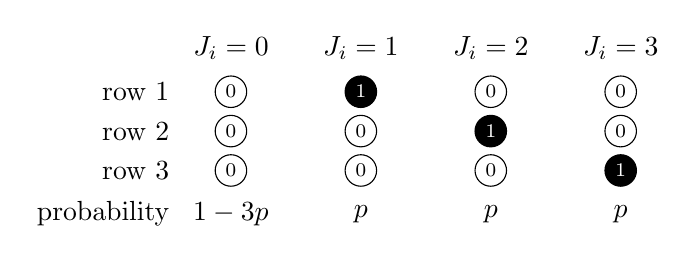
\begin{tikzpicture}[x=1.65cm,y=0.5cm,
  bit/.style={circle,draw,minimum size=4mm,inner sep=0pt},
  present/.style={bit,fill=black,text=white}]
  \foreach \x/\y in {0/1,0/2,0/3,1/1,1/2,2/1,2/3,3/2,3/3}
    \node[bit] at (\x,\y) {\scriptsize 0};
  \foreach \x/\y in {1/3,2/2,3/1}
    \node[present] at (\x,\y) {\scriptsize 1};
  \node at (0,4.1) {$J_i=0$};
  \node at (1,4.1) {$J_i=1$};
  \node at (2,4.1) {$J_i=2$};
  \node at (3,4.1) {$J_i=3$};
  \node at (0,-0.1) {$1-3p$};
  \foreach \x in {1,2,3} {\node at (\x,-0.1) {$p$};}
  \node[anchor=east] at (-0.4,3) {row 1};
  \node[anchor=east] at (-0.4,2) {row 2};
  \node[anchor=east] at (-0.4,1) {row 3};
  \node[anchor=east] at (-0.4,-0.1) {probability};
\end{tikzpicture}
\caption{One coordinate of the sparse coupling, illustrated with three
rows and $3p<1$. Each row contains this coordinate with probability $p$;
the union contains it with probability $3p$. Making these choices
independently across coordinates gives the required product laws.}
\label{fig:coupling}
\end{figure}


Define
\[
\mathcal F
=\{D_1\cup\cdots\cup D_L:D_1,\ldots,D_L\in\mathcal D\}.
\]
On the event in~\eqref{eq:all-good-rows}, the union $R$ belongs to
$\mathcal F$. Hence
\[
\mu_q(\mathcal F)=\mathbb P(R\in\mathcal F)
\ge\frac{31}{32}\ge\frac12.
\]
Grouping a tuple of $32L$ members of $\mathcal D$ into 32 groups of
size $L$, or conversely expanding 32 members of $\mathcal F$, shows that
the possible unions agree exactly. Thus
\[
E_{32}(\mathcal F)=E_{32L}(\mathcal D)=E_k(\mathcal D).
\]
Proposition~\ref{prop:half-density} makes this family $(q/L)$-small.
Since $q/L=p$, this is the required conclusion.

\medskip
\noindent\emph{Case 2: $Lp\ge1$.}
Set
\[
t=\frac{p-1/L}{1-1/L}\in[0,1).
\]
At each coordinate $i$, choose a mandatory row uniformly among the $L$
rows. Include $i$ in that row, and, conditional on this choice, include
it independently in each other row with probability $t$.
Make these choices independently across coordinates. For each fixed
row $j$,
\[
\mathbb P(i\in R_j)
=\frac1L+\left(1-\frac1L\right)t=p,
\]
and the coordinates of $R_j$ are independent. Thus each $R_j$ again has
law $\mu_p$, while the union of all rows is $[N]$ in every outcome.

By~\eqref{eq:all-good-rows}, some outcome has all $L$ rows in
$\mathcal D$. These rows cover $[N]$. Repeating the resulting tuple
32 times gives exactly $k$ members of $\mathcal D$ with full union.
Consequently $E_k(\mathcal D)=\varnothing$, which is covered at cost
zero by the empty family. This construction also covers the boundary
$Lp=1$, when $t=0$.
\end{proof}

\begin{thebibliography}{99}

\bibitem{AscoliEtAl26}
Ruben Ascoli, Xiaoyu He, Jinyoung Park, and Michel Talagrand,
\emph{A reformulation of the discrete Convexity Conjecture via
$k$-thresholds},
arXiv:2608.11183v1, 2026.
\href{https://arxiv.org/abs/2608.11183v1}{arXiv:2608.11183v1}.

\bibitem{EllisFilmusFriedgut12}
David Ellis, Yuval Filmus, and Ehud Friedgut,
\emph{Triangle-intersecting families of graphs},
Journal of the European Mathematical Society \textbf{14} (2012),
no.~3, 841--885.
\href{https://doi.org/10.4171/JEMS/320}{doi:10.4171/JEMS/320}.

\bibitem{FischerPerson25}
Thomas Fischer and Yury Person,
\emph{Further remarks on fractional vs. expectation thresholds},
arXiv:2505.21782v1, 2025.
\href{https://doi.org/10.48550/arXiv.2505.21782}{doi:10.48550/arXiv.2505.21782}.

\bibitem{Friedgut08}
Ehud Friedgut,
\emph{On the measure of intersecting families, uniqueness and stability},
Combinatorica \textbf{28} (2008), no.~5, 503--528.
\href{https://doi.org/10.1007/s00493-008-2318-9}{doi:10.1007/s00493-008-2318-9}.

\bibitem{HuaSongTudose26}
Dongming (Merrick) Hua, Antoine Song, and Stefan Tudose,
\emph{On Talagrand's Convexity Conjecture},
arXiv:2605.10908v2, 2026.
\href{https://arxiv.org/abs/2605.10908v2}{arXiv:2605.10908v2}.

\bibitem{Li26}
Chen Li,
\emph{On $p$-spread measures},
arXiv:2609.08967v1, 2026.
\href{https://arxiv.org/abs/2609.08967v1}{arXiv:2609.08967v1}.

\bibitem{ODonnell14}
Ryan O'Donnell,
\emph{Analysis of Boolean Functions},
Cambridge University Press, Cambridge, 2014.
Author's corrected text, 2021:
\href{https://arxiv.org/abs/2105.10386v1}{arXiv:2105.10386v1}.

\bibitem{OpenAIThreshold26}
OpenAI,
\emph{Integral and fractional expectation thresholds are equivalent},
OpenAI Math Release preprint
\href{https://github.com/openai/math/blob/main/preprints/Integral-and-fractional-expectation-thresholds-are-equivalent-September-23-2026/paper.pdf}{OAI:Integral-and-fractional-expectation-thresholds-are-equivalent-September-23-2026},
2026.

\bibitem{Park26}
Jinyoung Park,
\emph{A dimension-free comparison between expectation thresholds and
fractional expectation thresholds},
arXiv:2609.14681v1, 2026.
\href{https://arxiv.org/abs/2609.14681v1}{arXiv:2609.14681v1}.

\bibitem{ParkPham24}
Jinyoung Park and Huy Tuan Pham,
\emph{On a conjecture of Talagrand on selector processes and a consequence
on positive empirical processes},
Annals of Mathematics \textbf{199} (2024), no.~3, 1293--1321.
\href{https://doi.org/10.4007/annals.2024.199.3.6}{doi:10.4007/annals.2024.199.3.6}.

\bibitem{Talagrand10}
Michel Talagrand,
\emph{Are many small sets explicitly small?},
Proceedings of the Forty-Second ACM Symposium on Theory of Computing,
ACM, New York, 2010, 13--36.
\href{https://doi.org/10.1145/1806689.1806693}{doi:10.1145/1806689.1806693}.

\bibitem{Talagrand21}
Michel Talagrand,
\emph{Upper and Lower Bounds for Stochastic Processes:
Decomposition Theorems},
2nd ed., Ergebnisse der Mathematik und ihrer Grenzgebiete, 3.~Folge,
vol.~60, Springer, Cham, 2021.
\href{https://doi.org/10.1007/978-3-030-82595-9}{doi:10.1007/978-3-030-82595-9}.

\end{thebibliography}

\end{document}
